\section{Введение}
\subsection{Цели работы} 
\begin{itemize}
    \item Ознакомление с методами получения и анализа поляризованного света.
\end{itemize}

\subsection{Используемые приборы}
\begin{itemize}
    \item Оптическая скамья с осветителем;
    \item Зелёный светофильтр;
    \item Два поляроида;
    \item Чёрное зеркало;
    \item Полированная эбонитовая пластинка;
    \item Слюдяные пластинки разной толщины;
    \item Пластинки в 1/4 и 1/2 длины волны;
    \item Пластинка в одну длину волны для зеленого цвета (пластинка чувствительного оттенка)
\end{itemize}

\subsection{Теоретическая часть}

\subsubsection{Определение направления разрешённой плоскости колебаний
поляроида.}
Свет является электромагнитной волной, где вектор напряжённости электрического поля \( \mathbf{E} \) колеблется в определённой плоскости. Поляризация — явление упорядочивания направлений колебаний вектора \( \mathbf{E} \). Поляроиды — оптические устройства, пропускающие свет только с колебаниями в одном выделенном направлении (разрешённая плоскость).


При падении света на границу раздела сред под \textbf{углом Брюстера} \( \theta_B \), отражённый луч становится полностью поляризованным с колебаниями, параллельными поверхности (правило «иголки»). Угол Брюстера связан с коэффициентом преломления \( n \) материала:
\begin{equation}
    \tan\theta_B = n
\end{equation}


Для определения разрешённой плоскости поляроида используется чёрное зеркало. Последовательность действий:
\begin{enumerate}
    \item Поляроид и зеркало вращают до минимума интенсивности отражённого луча.
    \item При угле Брюстера вектор \( \mathbf{E} \) в падающем свете должен лежать в плоскости падения.
    \item По углу поворота зеркала вычисляют \( \theta_B \), а затем \( n \).
\end{enumerate}

\textbf{Важно:} минимальная интенсивность достигается только при одновременном выполнении двух условий — падение под \( \theta_B \) и совпадение плоскости колебаний с плоскостью падения.


\textbf{Эллиптическая поляризация}

Эллиптически поляризованный свет образуется при сложении двух линейно поляризованных волн с взаимно перпендикулярными направлениями колебаний и определённым сдвигом фаз. Для его получения используют \textbf{двоякопреломляющие пластинки} с двумя главными направлениями ($x$ и $y$), вдоль которых волны распространяются с разными скоростями.

\begin{figure}[H]
    \centering
    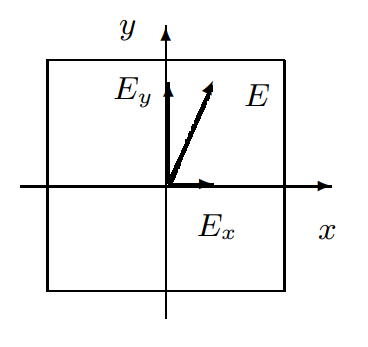
\includegraphics[width=0.4\linewidth]{pictures/2.png}
    \caption{Разложение линейно
поляризованного света по
главным направлениям
двоякопреломляющей
пластинки}
    \label{fig:enter-label}
\end{figure}

\textbf{Двоякопреломляющие пластинки}

\begin{itemize}
    \item Главные направления пластинки соответствуют осям эллипсоида диэлектрической проницаемости.
    \item Падающий линейно поляризованный свет раскладывается на компоненты $E_x$ и $E_y$ вдоль главных направлений.
    \item Разность хода между компонентами после прохождения пластинки толщиной $d$:
    \begin{equation}
        \Delta \phi = \frac{2\pi}{\lambda} \cdot d \cdot (n_x - n_y),
    \end{equation}
    где $n_x$, $n_y$ — показатели преломления для главных направлений.
\end{itemize}

\textbf{Частные случаи сдвига фаз}

\begin{enumerate}
    \item \textbf{Пластинка $\lambda$} ($\Delta \phi = 2\pi$): 
    Выходной свет остаётся линейно поляризованным с исходным направлением колебаний.
    
    \item \textbf{Пластинка $\lambda/2$} ($\Delta \phi = \pi$): 
    Направление колебаний поворачивается на угол $2\alpha$ относительно главных осей пластинки (зеркальное отражение).
    
    \item \textbf{Пластинка $\lambda/4$} ($\Delta \phi = \pi/2$): 
    При $E_x = E_y$ возникает круговая поляризация; в общем случае — эллиптическая поляризация.
\end{enumerate}

\begin{figure}[H]
    \centering
    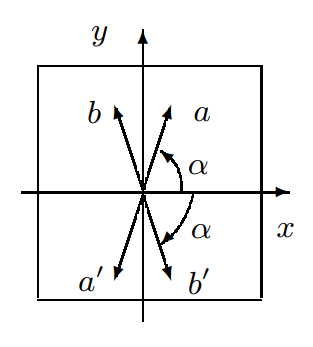
\includegraphics[width=0.4\linewidth]{pictures/3.png}
    \caption{Поворот
направления колебаний с
помощью пластинки в $\lambda/2$}
    \label{fig:enter-label}
\end{figure}

\textbf{Примечание:} свойства пластинок зависят от длины волны. Для немонохроматического света наблюдаются различные эллипсы поляризации для разных спектральных компонент.

\subsubsection{Анализ эллиптически поляризованного света}
Анализ включает два этапа:
\begin{enumerate}
    \item Определение \textbf{главных осей эллипса} поляризации с помощью анализатора (поляроида) — вращением анализатора фиксируют положения максимума и минимума интенсивности света.
    \item Установление \textbf{направления вращения вектора} \( \mathbf{E} \) с использованием пластинки \( \lambda/4 \).
\end{enumerate}

\textbf{Роль пластинки \( \lambda/4 \)}

\begin{itemize}
    \item Главные направления пластинки (\( x \) и \( y \)) совмещают с осями эллипса. При этом:
    \begin{equation}
        n_x < n_y \quad \text{(волна } E_x \text{ распространяется быстрее)}.
    \end{equation}
    
    \item Пластинка изменяет сдвиг фаз между \( E_x \) и \( E_y \):
    \begin{itemize}
        \item Исходный сдвиг для эллиптической поляризации: \( \Delta\phi = \pi/2 \).
        \item После пластинки \( \lambda/4 \): \( \Delta\phi \rightarrow 0 \) или \( \pi \).
    \end{itemize}
    
    \item Результирующий свет становится \textbf{линейно поляризованным}. Направление колебаний зависит от начального вращения \( \mathbf{E} \):
    \begin{itemize}
        \item \textbf{Против часовой стрелки}: колебания во II и IV квадрантах.
        \item \textbf{По часовой стрелке}: колебания в I и III квадрантах.
    \end{itemize}
\end{itemize}

\textbf{Процедура определения вращения}

\begin{enumerate}
    \item Совместить оси пластинки \( \lambda/4 \) с осями эллипса.
    \item Проанализировать направление колебаний выходного линейно поляризованного света с помощью поляроида.
    \item По положению вектора \( \mathbf{E} \) (квадранты) определить направление вращения.
\end{enumerate}

Метод требует знания соотношения \( n_x \) и \( n_y \) для пластинки \( \lambda/4 \). Для немонохроматического света анализ усложняется из-за зависимости \( \Delta\phi \) от \( \lambda \).

\subsubsection{Пластинка чувствительного оттенка}]
Пластинка чувствительного оттенка — кристаллическая пластинка толщиной $\lambda$ для зелёного света ($\lambda = 560 \, \text{нм}$). Её главные направления обозначены в форме стрелы (рис. 1), где ось стрелы соответствует направлению с \textbf{большей скоростью} распространения света ($n_x < n_y$).

\begin{figure}[H]
    \centering
    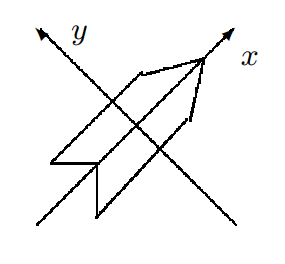
\includegraphics[width=0.4\textwidth]{pictures/1.png} % Шаблон для вставки изображения
    \caption{Пластинка чувствительного оттенка. Главное направление указано стрелкой.}
    \label{fig:sensitive_plate}
\end{figure}

\textbf{Определение направления большей скорости}

\begin{itemize}
    \item При размещении пластинки между \textbf{скрещенными поляроидами} под углом к их осям, она окрашивается в \textbf{лилово-красный} цвет. 
    \item Зелёный свет ($\lambda = 560 \, \text{нм}$) не меняет поляризации и блокируется вторым поляроидом.
    \item Красная и фиолетовая компоненты приобретают эллиптическую поляризацию и частично проходят, формируя дополнительный к зелёному цвет.
\end{itemize}

\textbf{Совместное использование с пластинкой $\lambda/4$}

\begin{enumerate}
    \item При совпадении главных направлений пластинки $\lambda/4$ и пластинки чувствительного оттенка:
    \begin{equation}
        \Delta = \frac{5\lambda}{4} \quad \text{(для зелёного света)}, \quad \Delta = \lambda \quad \text{(для красного света)}.
    \end{equation}
    Красный свет гасится, проходящий свет становится \textbf{зеленовато-голубым}.
    
    \item При перпендикулярном расположении главных направлений:
    \begin{itemize}
        \item Гасится фиолетово-голубая компонента.
        \item Проходящий свет имеет \textbf{оранжево-жёлтую} окраску.
    \end{itemize}
\end{enumerate}

\textbf{Практическое применение}

Изменение цвета позволяет определить:
\begin{itemize}
    \item Соответствие главных направлений пластинки $\lambda/4$ большей/меньшей скорости.
    \item Направление вращения вектора $\mathbf{E}$ в эллиптически поляризованном свете.
\end{itemize}

Метод работает только для монохроматического света. Для белого света наблюдаются сложные цветовые эффекты из-за зависимости $\Delta\phi(\lambda)$.

\subsubsection{Интерференция поляризованных лучей}
При размещении двоякопреломляющей пластинки между скрещенными поляроидами возникает окрашивание, обусловленное интерференцией когерентных волн. Схема эксперимента показана на рис. \ref{r4}.

\begin{figure}[H]
    \centering
    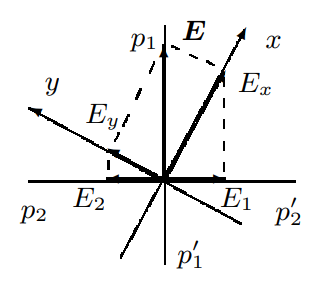
\includegraphics[width=0.4\textwidth]{pictures/4.png} % Шаблон для вставки изображения
    \caption{Схема интерференции поляризованных лучей: \( p_1p_1' \) — направления поляризатора и анализатора, \( x,y \) — главные направления пластинки.}
    \label{r4}
\end{figure}

\textbf{Условия интерференции}

\begin{itemize}
    \item Волны \( E_x \) и \( E_y \) после пластинки \textbf{когерентны}, но не интерферируют из-за взаимной перпендикулярности.
    \item Анализатор проектирует \( E_x \) и \( E_y \) на общее направление \( p_2p_2' \), формируя волны \( E_1 \) и \( E_2 \) с \textbf{одинаковой поляризацией}.
    \item Результирующая интенсивность определяется разностью фаз:
    \begin{equation}
        \Delta\phi = \frac{2\pi}{\lambda} \cdot d \cdot (n_x - n_y),
    \end{equation}
    где \( d \) — толщина пластинки.
\end{itemize}

\textbf{Цветовые эффекты}

\begin{enumerate}
    \item При освещении \textbf{белым светом} пластинка кажется окрашенной из-за зависимости \( \Delta\phi(\lambda) \).
    \item \textbf{Поворот пластинки} между скрещенными поляроидами:
    \begin{itemize}
        \item Не изменяет цвет (сохранение \( \Delta\phi \)).
        \item Интенсивность света обращается в нуль 4 раза за полный оборот (при совпадении \( x,y \) с \( p_1,p_2 \)).
    \end{itemize}
    
    \item \textbf{Поворот анализатора} на \( 90^\circ \) (совмещение \( p_1 \) и \( p_2 \)):
    \begin{itemize}
        \item Добавляет фазовый сдвиг \( \pi \) для всех \( \lambda \).
        \item Цвет пластинки меняется на \textbf{дополнительный}.
    \end{itemize}
\end{enumerate}

\textbf{Ключевые наблюдения}

\begin{itemize}
    \item Окрашивание исчезает при использовании монохроматического света.
    \item Эффекты объясняются интерференцией проекций \( E_x \) и \( E_y \) на ось анализатора.
    \item Явление используется для анализа напряжений в материалах и кристаллографических исследований.
\end{itemize}

\textbf{Примечание:} Для количественного анализа необходимо учитывать дисперсию двоякопреломления \( n_x(\lambda) - n_y(\lambda) \).


\subsection{Экспериментальная установка}

\begin{figure}
    \centering
    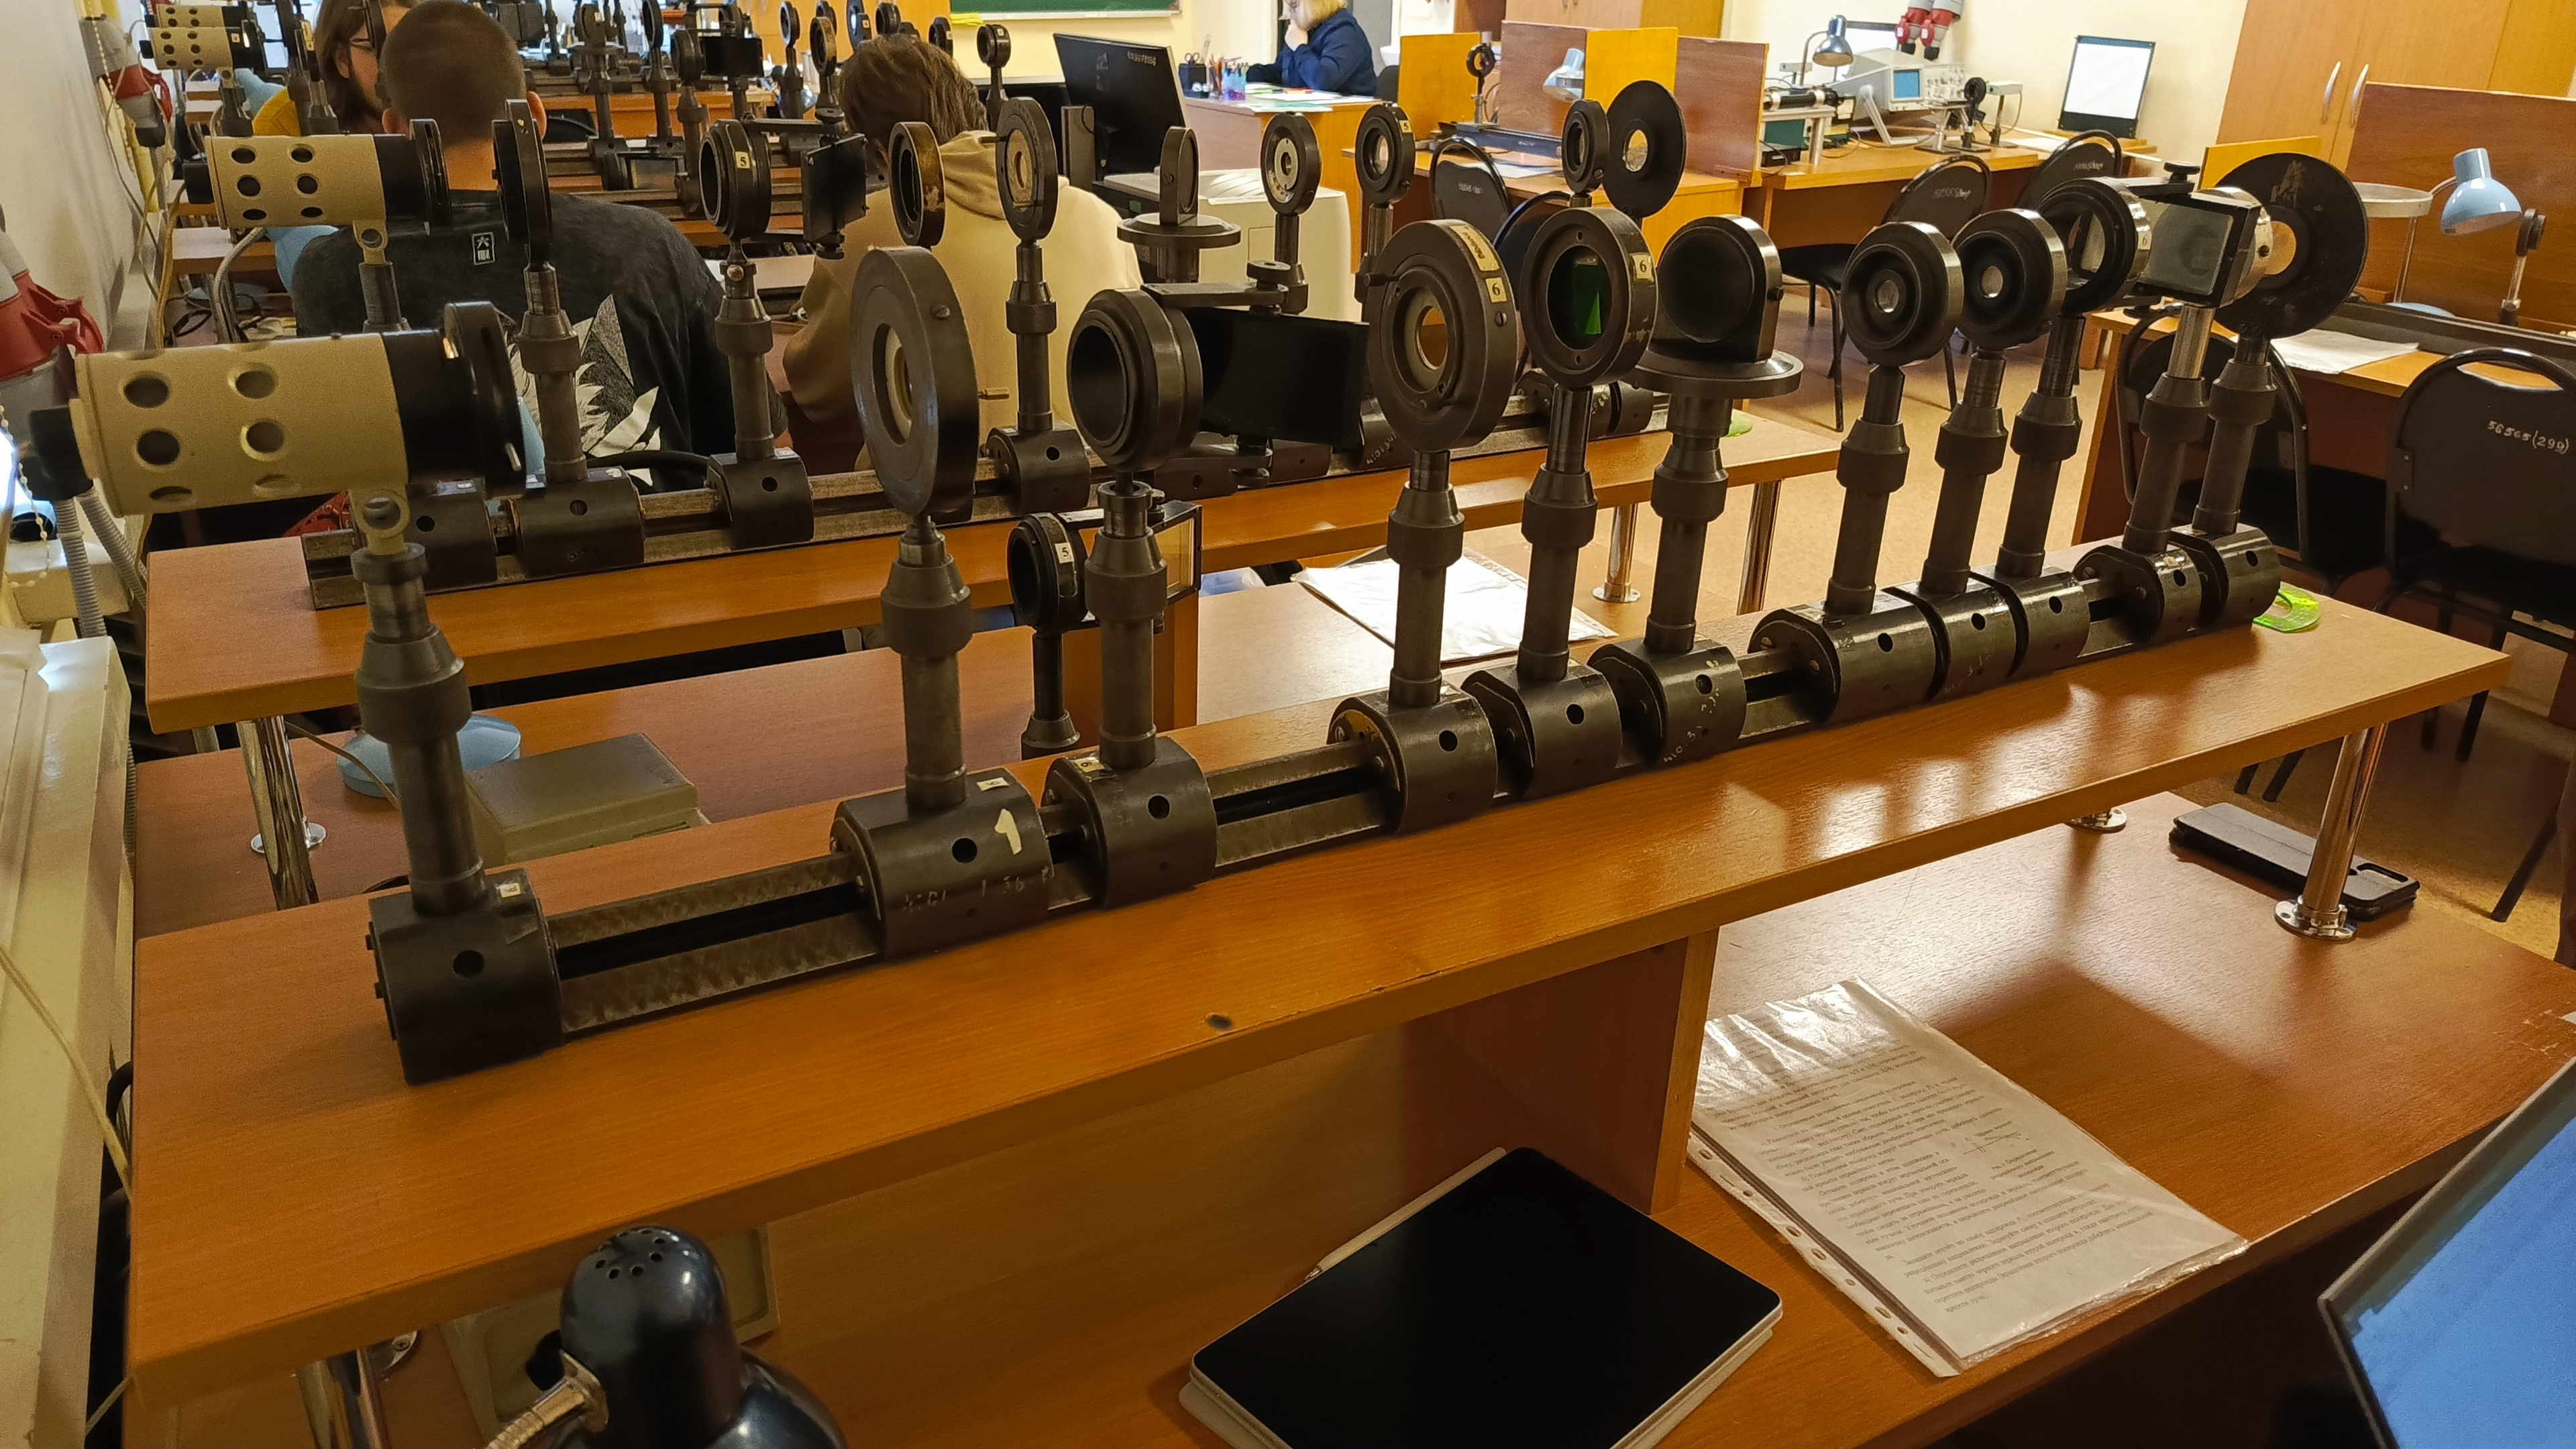
\includegraphics[width=1\linewidth]{pictures/IMG_20250315_092255_086.jpg}
    \caption{Моя прелесть}
    \label{fig:enter-label}
\end{figure}

